\chapter{Introduction}\label{Introduction}

Encrypted Client Hello (ECH) is a proposed extension to the Transport Layer Security protocol version 1.3 (TLS 1.3) which has begun to see implementation and adoption on the Internet~\cite{ietf-tls-esni-18, tsiatsikas2022measuring, CF-ECH}. ECH seeks to allow encryption of the ClientHello message, which can contain potentially sensitive information such as the Server Name Indication (SNI) and Application-Layer Protocol Negotiation (ALPN) extensions. This is partially achieved through serving many private domains behind a common provider to form an anonymity set that conceals the true domain requested by the client.

Due to this, ECH introduces significant centralisation to the Internet. This paper presents a practical model for the distributed deployment of ECH amongst several co-operating TLS servers, where each server operates both as the origin server of its own domains as well as an ECH provider for other participating servers. The model addresses a number of implementation challenges, predominately related to ensuring the security of the protocol is not compromised and minimising the performance impact to the connection while strengthening service availability.

Included in this paper is a review of the background technology and concepts relevant to the discussion of the deployment model. This is followed by a study of the model's design and the complications which influenced it. We then see how this design can be implemented within a practical scenario and discuss some of its deployment considerations. In the subsequent chapter, an analysis and criticism of both the results taken from this implementation and the design as a whole is used to assess the quality of the solution. Finally, I conclude the report with a summary of the work completed and delineate where future contributions could best benefit the further development of the deployment model.









\section{Motivation}

Nottingham has previously cautioned against the introduction of centralisation through Internet standards~\cite{rfc9518}. Of particular relevance to ECH is his highlight of the adverse effect centralisation can have on infrastructure resilience and service availability through reliance on a single entity. This is especially detrimental to ECH where the effectiveness of its anonymity set grows with the number of private domains served by a single provider. Nottingham also writes on susceptibility of centralisation to stifle ``permissionless'' innovation and induce an unhealthy monoculture, which may result in less overall technological progress and robustness of the ECH protocol.

Additionally, allowing entirely independent servers to co-operate from across the Internet to provide ECH support for each other enables several distinct organisations to work together to offer improved privacy for their users without the requirement for co-located servers nor the dependence of any on the availability on another. Consider here global networks of whistleblower services, investigative journalists and human rights non-profit organisations who share an interest in protecting the confidentiality of their members and users from persecution and retaliation.

For these reasons, the development of a model for the distributed deployment of ECH across several co-operating providers is a key step towards its broad adoption throughout the Internet and its application within more elaborate scenarios.









\section{Project Objectives}

The objectives of this research project can be summarised with the following question: ``How can Encrypted Client Hello be deployed fairly amongst co-operating Transport Layer Security servers to reduce network centralisation without compromising the security of the protocol?'' This task is composed of the following objectives:

\begin{description}
	\item[1. Identify principal challenges and appropriate solutions.] Before development can begin proper, we must first understand the environment the system would operate in and explore the technical and logistical issues it might face to determine the dominant criteria for design. We accomplish this through research and experimentation of the functioning of the protocol and its surrounding technologies.
	\item[2. Design, evalute and contrast deployment models.] An iterative development process is used to produce a series of incrementally improved skeletal prototypes, with the goal to rapidly design and test for functionality guided by the design criteria and results of previous work as heuristics.
	\item[3. Analyse model implementatons through simulation.] Promising design solutions are fleshed out into full implementations within deterministic, reproducible and quantifiable simulated environments, where security and performance implications can be easily isolated and compared. This allows for these effects to be consistently measured against implementations based on a centralised ECH deployment model or with ECH support disabled entirely. It is also expected that unforeseeable practical challenges and considerations are to be unveiled during this work.
	\item[4. Conclude findings and present results.] The data collected and learnings gained during analysis of model implementations is to be compiled into a report on the overall effectiveness of distributed ECH deployment and recommendations for future researchers and service operators. Of particular use here is a study on the effect distributed ECH has on performance when compared to other implementations.
\end{description}

In preparation of these objectives, I produced the Gantt chart included in Fig.~\ref{gantt_chart_figure} to help gauge my progress during the four months of work. While in the final result I have found more emphasis has been placed on implementation, the overall structure of the timeline has been followed reasonable well.

\begin{figure}[ht]
\centerline{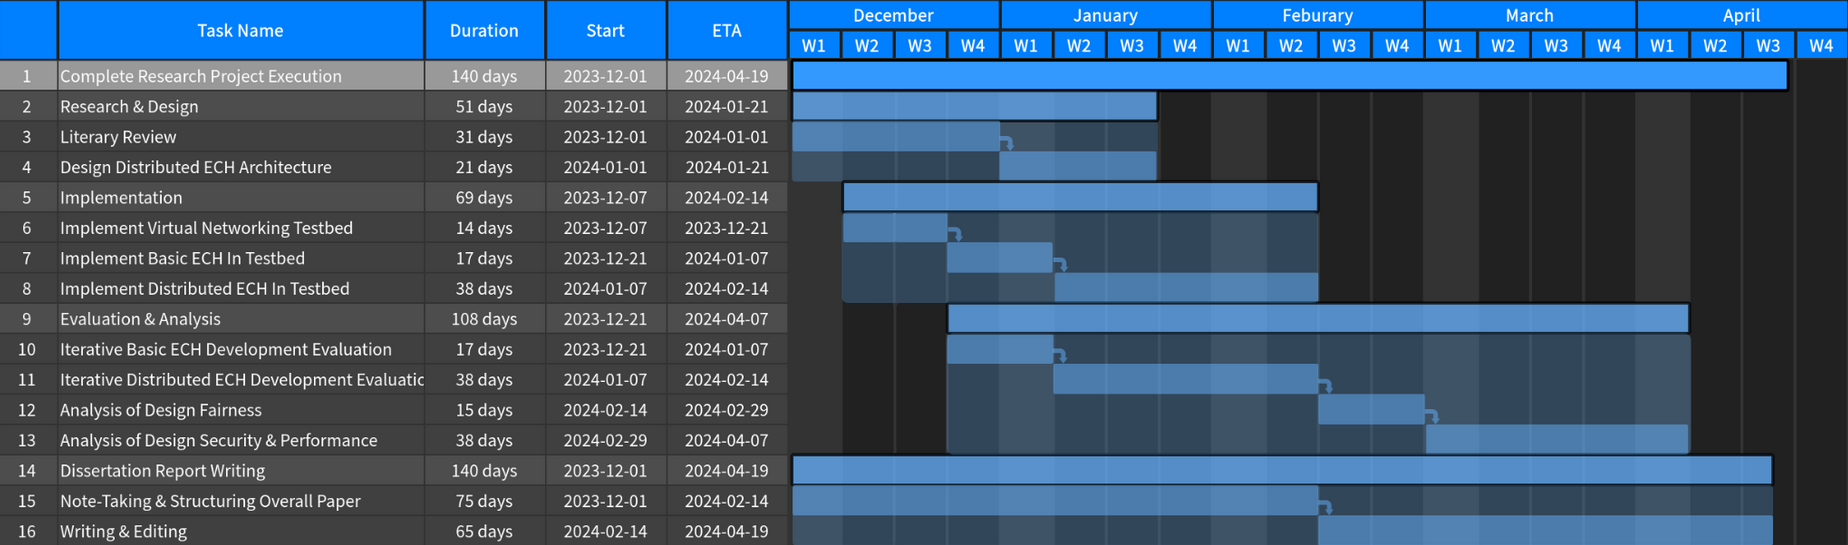
\includegraphics[width=160mm]{images/gantt.png}}
\caption[Project timeline]{Predicted timeline of project as of the 7\textsuperscript{th} of December, 2023.}
\label{gantt_chart_figure}
\end{figure}









\section{Research Contributions}

This work provides evidence for the viability of the distributed deployment of ECH between co-operative TLS servers. It supports its argument that the deployment model presented does not compromise the security of the protocol and minimises impact to network performance though analysis of the data produced by implementations within simulated networking environments. Additionally, an evaluation of several traffic masking and normalisation techniques is given to serve as the bases for further work on disrupting traffic correlation attacks applicable to ECH and elsewhere. Finally, the delivered project may also contribute academic value as a deterministic, reproducible tutorial on the deployment and operation of ECH using commonplace software and tooling.
